% chapter3_07.tex -- de (German)
% audio parameters
\section{Konfigurationsdateien im Verzeichnis \filenam{RPi-Jukebox-RFID/settings}}
Das Unterverzeichnis filenam{/home/pi/RPi-Jukebox-RFID/settings} enth�lt
einige Konfigurationsdateien, in denen das Verhalten der {\Bezeichnung}
eingestellt und angepasst werden kann. Der Dateiinhalt bestaht dabei nur
aus dem gew�nschten Parameter. Die Funktion wird durch den Dateinamen
bestimmt und ist in den jeweiligen Python- \bzw Shellskripten fest
hinterlegt, siehe\\
\begin{smaller}\url{https://github.com/MiczFlor/RPi-Jukebox-RFID/wiki/CONFIGURE-stretch#create-settings-for-audio-playout}\end{smaller}

\subsection{Audioeinstellungen}
Die folgenden Kommandos legen im Verzeichnis
\filenam{/home/pi/RPi-Jukebox-RFID/settings} kleine Textdateien an, die
das Verhalten der Taster \textit{volume up} und \textit{volume down}
konfigurieren. Ferner kann die maximale Lautst�rke begenzt werden:\\
\cmdPi{echo \dq Master\dq\ > /home/pi/RPi-Jukebox-RFID/settings/Audio\_iFace\_Name}\\
\cmdPi{echo \dq 3\dq\ > /home/pi/RPi-Jukebox-RFID/settings/Audio\_Volume\_Change\_Step}\\
\cmdPi{echo \dq 100\dq\ > /home/pi/RPi-Jukebox-RFID/settings/Max\_Volume\_Limit}

MP3-Dateien f�r Startup und Shutdown kopieren:\\
\cmdPi{\begin{scriptsize}cp /home/pi/RPi-Jukebox-RFID/misc/sampleconfigs/startupsound.mp3.sample\\ /home/pi/RPi-Jukebox-RFID/shared/startupsound.mp3\end{scriptsize}}\\
\cmdPi{\begin{scriptsize}cp /home/pi/RPi-Jukebox-RFID/misc/sampleconfigs/shutdownsound.mp3.sample\\ /home/pi/RPi-Jukebox-RFID/shared/shutdownsound.mp3\end{scriptsize}}

\subsection{automatische Abschaltung bei Nichtbenutzung}
Gerade bei Kindern ist es sinnvoll, die {\Bezeichnung} nach einiger Zeit
der Nichtverwendung automatisch abzuschalten, um die Akkulaufzeit zu
verl�ngern. Der angegebene Wert ist inaktive Zeit in Minuten
\textit{ab dem Beenden der \software{mpd}-Playlist}, bevor sich die Box
automatisch abschaltet. Der Wert 0 deaktiviert diese Funktion.\\ 
\cmdPi{echo \dq 0\dq\ > /home/pi/RPi-Jukebox-RFID/settings/Idle\_Time\_Before\_Shutdown}

Ein automatisches Abschalten der {\Bezeichnung} nach 15 Minuten
Nichtbenutzung erreicht man alternativ durch:\\
\cmdPi{echo \dq 15\dq\ > /home/pi/RPi-Jukebox-RFID/settings/Idle\_Time\_Before\_Shutdown}%\comment{Alternative}

\subsection{Was soll beim wiederholten Auflegen einer {\Karte} passieren?}
Quelle:\\
\url{https://github.com/MiczFlor/RPi-Jukebox-RFID/wiki/MANUAL#second-swipe}

In der Datei \filenam{/home/pi/RPi-Jukebox-RFID/settings/Second\_Swipe}
wird festgelegt, was beim wiederholten Auflegen derselben {\Karte}
passieren soll. Dazu wird in diese Datei das entsprechende Schl�sselwort
aus folgender Liste eingetragen:

\begin{table}[h]
\centering
\renewcommand{\arraystretch}{1.25}
\begin{tabular}{|p{0.15\textwidth}|p{0.80\textwidth}|}
\hline
\textbf{Schl�sselwort}	&	\textbf{Funktion}\\
\hline
\texttt{RESTART}		&	Neustart der aktiven Playlist von Anfang an\\
\hline
\texttt{PAUSE}			&	Umschalten zwischen \textit{Play/Pause}\\
\hline
\texttt{SKIPNEXT}		&	Zum n�chsten Titel aus der Playlist springen\\
\hline
\texttt{NOAUDIOPLAY}	&	Keine Beeinflussung der Audiowiedergabe\\
\hline
\end{tabular}
\vspace{0.5cm}
\caption{Verhalten bei wiederholtem Auflegen derselben \Karte}
\label{tab:second_swipe}
\end{table}

Bei meiner Box habe ich mich f�r den Eintrag \texttt{PAUSE}
entschieden.\\
\cmdPi{nano /home/pi/RPi-Jukebox-RFID/settings/Second\_Swipe}\\
\stdout{PAUSE}

\begin{bclogo}[logo = \bclampe, noborder = true]{Hinweis}
In der Webapp ist die Einstellung sicherer...
\end{bclogo}

\begin{figure}[h]
\centering
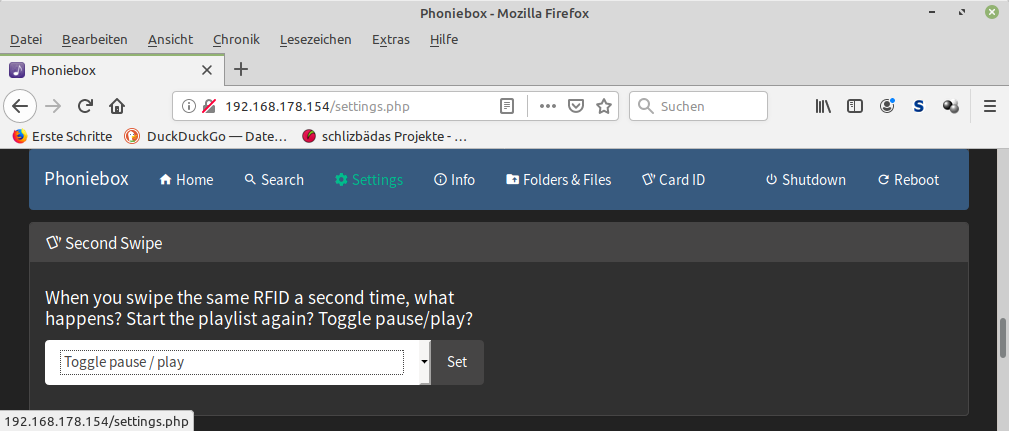
\includegraphics[width=0.90\textwidth]{/software/Second_Swipe.png}
\caption{Einstellung des Verhaltens bei wiederholtem Auflegen derselben {\Karte} �ber die WebApp}
\end{figure}
